\chapter{Resultados  Preliminares}
\label{chap:resultados_discussao}

%--------------------------------------------------------
\section{Resultados} 
\label{sec:cap6_resultados}

Os testes iniciais foram aplicados ao conjunto de dados do \gls{ACDC}. Este conjunto de dados público já vem separado com 100 exames para treino e 50 para testes. A Figura \ref{fig:fig018} e \ref{fig:fig019} são exemplos de imagens de \gls{DCM} e \gls{HCM} capturadas na diástole, ambas com suas máscaras. Na Figura \ref{fig:fig020} temos uma imagem de coração em estado normal (\gls{NOR}).

\begin{figure}[htbp]
    \caption{Captura Diastólica DCM}
    \centering
    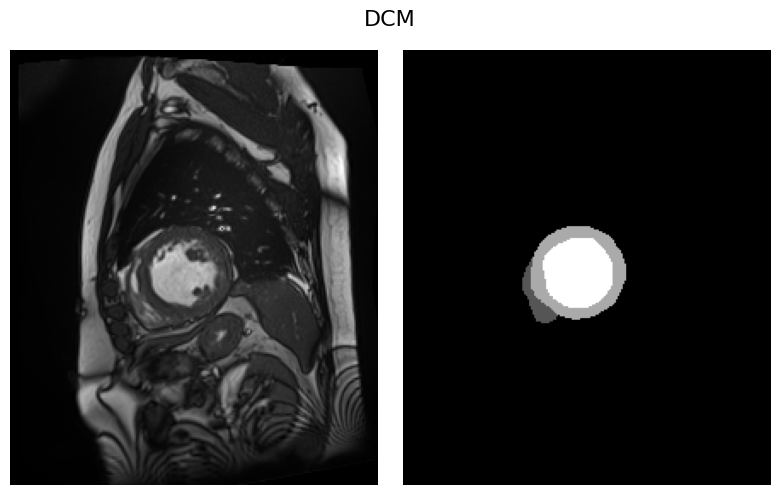
\includegraphics[width=0.65\textwidth]{figures/fig018.png}
    \caption{Fonte: Autor}
    \label{fig:fig018}
\end{figure}

\begin{figure}[htbp]
    \caption{Captura Diastólica de HCM}
    \centering
    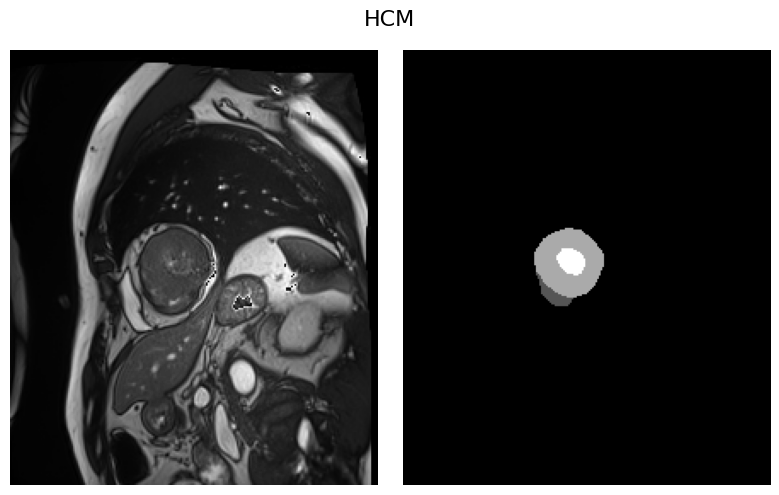
\includegraphics[width=0.65\textwidth]{figures/fig019.png}
    \caption{Fonte: Autor}
    \label{fig:fig019}
\end{figure}

\begin{figure}[htbp]
    \caption{Captura Diastólica NOR}
    \centering
    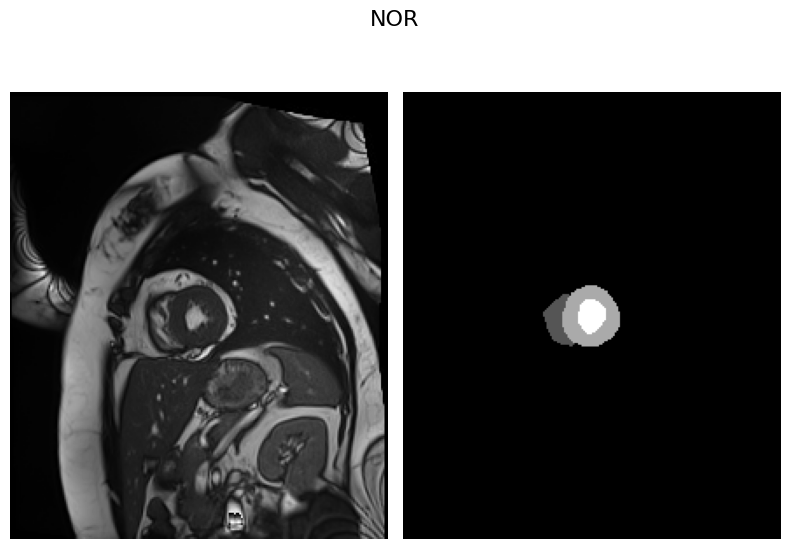
\includegraphics[width=0.65\textwidth]{figures/fig020.png}
    \caption{Fonte: Autor}
    \label{fig:fig020}
\end{figure}

Os resultados foram obtidos aplicando a metodologia previamente apresentada, foi extraídas as \textit{features} radiômicas e profundas, após foi aplicado o F-Test para seleção de \textit{features} e o resultado concatenado. Por fim, o modelo de \textit{self-attention} foi aplicado, os hiperparâmetros utilizados são: taxa de aprendizado $0,0001$, otimizador \gls{Adam} e aproximadamente 300 épocas. As principais métricas calculadas são conferidas na Tabela \ref{tab:metrics}.

\begin{table}[hbtp]
    \centering
    \renewcommand{\arraystretch}{1} % default é 1 
    \begin{tabular}{|c|c|}
    \hline 
          \textbf{Métrica} & \textbf{Valor} \\ 
    \hline 
        Acurácia & 0.62 \\ 
    \hline 
        Precisão & 0.67 \\ 
    \hline 
        Revocação & 0.10 \\ 
    \hline 
        AUC & 0.63 \\ 
    \hline 
    \end{tabular} 
    \caption{Fonte: Autor}
    \label{tab:metrics}
\end{table}

A matriz de confusão é conferida Figura \ref{fig:fig016}.

\begin{figure}[htbp]
    \caption{Matriz de Confusão}
    \centering
    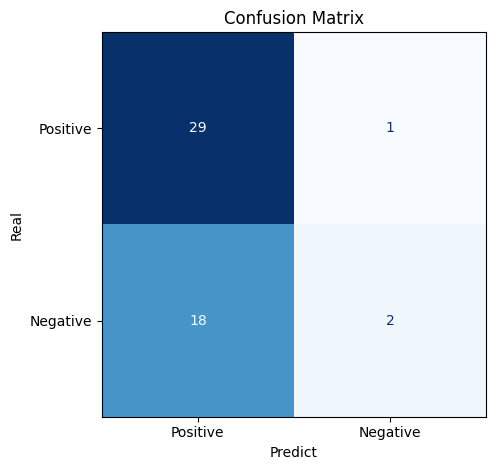
\includegraphics[width=0.55\textwidth]{figures/fig016.png}
    \caption{Fonte: Autor}
    \label{fig:fig016}
\end{figure}

Um gráfico ilustrativo da \gls{ROC} é visto na Figura \ref{fig:fig017}

\begin{figure}[htbp]
    \caption{ROC}
    \centering
    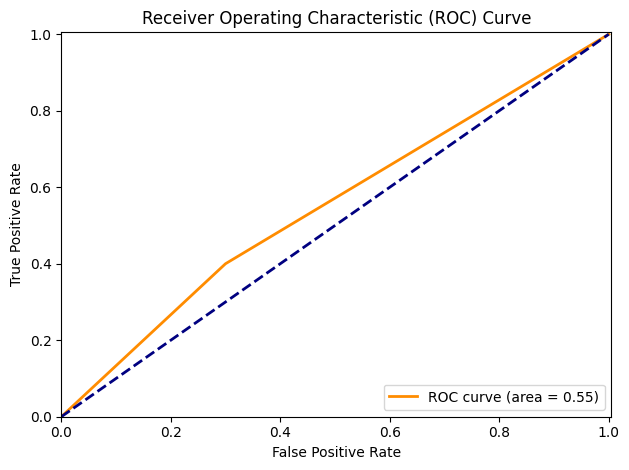
\includegraphics[width=0.75\textwidth]{figures/fig017.png}
    \caption{Fonte: Autor}
    \label{fig:fig017}
\end{figure}

%--------------------------------------------------------
\section{Conclusão dos Resultados} 
\label{sec:cap6_conclusãp_resultados}

Os resultados obtidos, diferente do trabalho similar aplicado à identificação de câncer no pulmão, obteve resultados pouco relevantes o que indica que há espaço para exploração e melhoria para o âmbito de \gls{CH}. Algumas, abordagens ainda são tidas em vista como manipular o seletor de \textit{features} e a sua quantidade, testar novos hiperparâmetros para os modelos, ao invés de ter um único módulo de \textit{self-attention}, aplicar vários em cascata, etc.


% %--------------------------------------------------------
% \subsection{Experimentos ACDC}
% \label{subsec:cap5_experimentos_acdc}



